% Concise academic version. Compile twice from this directory:
% pdflatex -interaction=nonstopmode -halt-on-error V4_model.tex
% Keep V4_structure.png beside this source.
\documentclass[11pt,a4paper]{article}
\usepackage[margin=22mm]{geometry}
\usepackage[T1]{fontenc}
\usepackage{newtxtext,newtxmath}
\usepackage{microtype}
\usepackage{graphicx}
\usepackage{amsmath}
\usepackage{array,booktabs}
\usepackage{caption}
\usepackage{titlesec}
\usepackage[hidelinks]{hyperref}
\hypersetup{pdftitle={},pdfauthor={},pdfsubject={V4 architecture and loss functions}}
\pagestyle{plain}
\raggedbottom
\setlength{\parindent}{1em}
\setlength{\parskip}{0pt}
\setlength{\emergencystretch}{1em}
\titlespacing*{\section}{0pt}{9pt plus 2pt minus 1pt}{5pt}
\titlespacing*{\subsection}{0pt}{6pt plus 1pt minus 1pt}{3pt}
\titleformat{\section}{\normalfont\large\bfseries}{\thesection}{0.7em}{}
\titleformat{\subsection}{\normalfont\normalsize\bfseries}{\thesubsection}{0.7em}{}
\newcommand{\loss}[1]{\mathcal L_{\mathrm{#1}}}
\newcommand{\mean}{\operatorname{mean}}
\newcommand{\BCE}{\operatorname{BCE}}
\newcommand{\Dice}{\operatorname{Dice}}
\newcommand{\GIoU}{\operatorname{GIoU}}
\captionsetup[table]{font=small,labelfont=bf,skip=5pt,hypcap=false}
\newcommand{\lossheading}[1]{\subsection{#1}}

\newenvironment{lossblock}[1]{%
  \par\addvspace{3pt}\noindent\begin{minipage}{\textwidth}%
  \lossheading{#1}%
}{\end{minipage}\par}

\begin{document}
\setlength{\abovedisplayskip}{5pt plus 1pt minus 1pt}
\setlength{\belowdisplayskip}{5pt plus 1pt minus 1pt}
\setlength{\abovedisplayshortskip}{3pt}
\setlength{\belowdisplayshortskip}{4pt}
\section{Model structure}
\noindent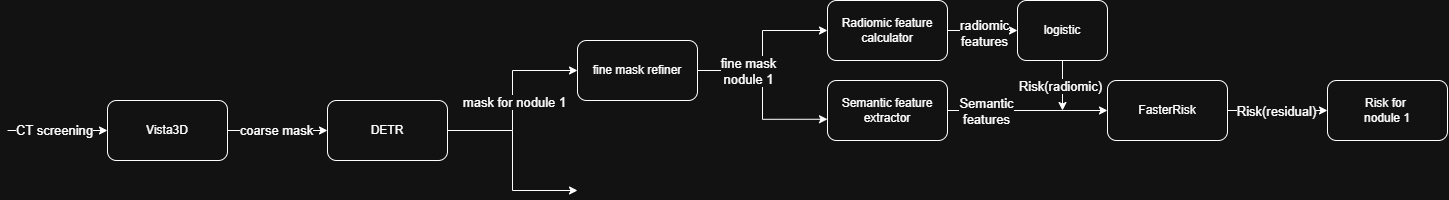
\includegraphics[width=\textwidth]{V4_structure.png}
\par\vspace{-3pt}

\section{Training objective}
V4 combines ten losses:
\[
  \loss{total}=\sum_{\ell=1}^{10}\lambda_\ell\loss{\ell},
\]
where $\loss{\ell}$ is a component loss and $\lambda_\ell$ is its weight.
Table~\ref{tab:weights} lists the weights used in joint training.

\begin{center}
\captionof{table}{Weights of the ten loss components.}
\label{tab:weights}
\renewcommand{\arraystretch}{1.0}
\begin{tabular*}{0.62\textwidth}{@{\extracolsep{\fill}}lr@{}}
\toprule
Loss component & Weight\\
\midrule
Box regression          & 5.0\\
Box GIoU                & 2.0\\
Coarse Dice             & 1.0\\
Coarse focal            & 1.0\\
Fine Dice               & 2.0\\
Fine focal              & 1.0\\
Missing-nodule penalty  & 2.0\\
Semantic supervision    & 1.0\\
Nodule malignancy       & 0.5\\
Scan-level risk         & 0.5\\
\bottomrule
\end{tabular*}
\end{center}

Averages use eligible training samples; fine-mask losses use only valid
ROI voxels. GT denotes ground truth, and ROI denotes region of interest.
Superscripts $c$ and $f$ indicate coarse and fine resolution.

\section{Loss components}

\begin{lossblock}{Box regression}
\[
  \loss{box}=\mean\bigl[|\widehat{\mathbf b}-\mathbf b|\bigr].
\]
Here $\widehat{\mathbf b}$ and $\mathbf b$ contain the predicted and GT box
centers and side lengths, normalized by the scan dimensions. The mean
is taken over matched nodules and their six coordinates.
This loss encourages accurate nodule location and size.
\end{lossblock}

\begin{lossblock}{Box GIoU}
\[
  \loss{GIoU}=\mean\bigl[1-\GIoU(\widehat B,B)\bigr].
\]
Here $\widehat B$ and $B$ are matched predicted and GT boxes.
GIoU measures their overlap and penalizes unused space in their smallest
enclosing box. Averaged across nodules, this loss encourages spatial
agreement even when the boxes initially do not overlap.
\end{lossblock}

\begin{lossblock}{Coarse Dice}
\[
  \loss{Dice}^{c}
  =\mean\left[1-\frac{2\sum_u p_u g_u}
                         {\sum_u p_u+\sum_u g_u}\right].
\]
Here $p_u$ is the predicted coarse foreground probability and $g_u$ is the
binary GT mask at voxel $u$. The sums cover the coarse grid, and the mean
covers matched nodules. This loss rewards overall foreground overlap
without letting the large background dominate.
\end{lossblock}

\begin{lossblock}{Coarse focal}
\[
  \loss{focal}^{c}
  =\mean\bigl[-\alpha_t(1-p_t)^2\log p_t\bigr].
\]
Here $p_t$ is the probability assigned to the correct voxel label:
$p$ for foreground and $1-p$ for background. The class weight $\alpha_t$
is $0.25$ for foreground and $0.75$ for background. The mean covers voxels
in matched coarse masks. The factor $(1-p_t)^2$ emphasizes difficult
voxels and reduces the influence of easy predictions.
\end{lossblock}

\begin{lossblock}{Fine Dice}
\[
  \loss{Dice}^{f}=\mean\bigl[1-\Dice(p^f,g^f)\bigr].
\]
Here $p^f$ and $g^f$ are the refined mask probabilities and cropped GT mask;
Dice is the same overlap ratio used for coarse segmentation. It is evaluated on
valid voxels and averaged over matched ROIs with sufficient GT coverage.
This loss encourages accurate local nodule shape and volume.
\end{lossblock}

\begin{lossblock}{Fine focal}
\[
  \loss{focal}^{f}=\mathrm{FL}_{+}+0.25\,\mathrm{FL}_{-}.
\]
Here $\mathrm{FL}_{+}$ and $\mathrm{FL}_{-}$ are the focal expression above,
averaged separately over valid voxels in matched positive ROIs and
unmatched hard-negative ROIs. Hard negatives receive all-background
targets. This loss refines difficult local details and suppresses spurious
masks in false candidates.
\end{lossblock}

\begin{lossblock}{Missing-nodule penalty}
\[
  \loss{miss}=-\mean\bigl[\log(oR_{\mathrm{fg}})\bigr],
  \qquad R_{\mathrm{fg}}=\frac{\sum_u g_u p_u}{\sum_u g_u}.
\]
Here $o$ is the matched query's object probability, $p_u$ is its coarse
mask probability, and $g_u$ is the binary GT mask.
The soft recall $R_{\mathrm{fg}}$ measures coverage of GT foreground.
The mean includes every retained GT nodule, independently of fine-ROI
coverage. This loss penalizes low detection confidence and missed
foreground, providing an explicit signal against missing nodules.
\end{lossblock}

\begin{lossblock}{Semantic supervision}
\[
  \loss{sem}
  =\mean_{i,j}\left[-\sum_{k=1}^{5}h_{ijk}\log\pi_{ijk}\right].
\]
Here $i$ indexes a valid matched nodule, $j$ a semantic attribute, and $k$
a rating from one to five. The target $h_{ijk}$ is the fraction of readers
assigning rating $k$, and $\pi_{ijk}$ is the predicted probability.
The six attributes are lobulation, margin, sphericity, spiculation,
subtlety, and texture. This loss learns interpretable attributes while
preserving disagreement among readers.
\end{lossblock}

\begin{lossblock}{Nodule malignancy}
\[
  \loss{nod}=\mean_{i,m}\bigl[\BCE(p_{im},y_i)\bigr],
  \qquad p_{im}=\sigma(a_i^{\mathrm{rad}}+c_{im}).
\]
Here $i$ indexes a valid matched nodule and $m$ a selected FasterRisk model.
The radiomics baseline logit is $a_i^{\mathrm{rad}}$, the semantic logit
correction is $c_{im}$, and $\sigma$ is the sigmoid function.
The combined malignancy probability $p_{im}$ is compared with the binary
GT label $y_i$ using binary cross-entropy (BCE).
With the baseline fixed during backpropagation, this loss trains semantic
features to explain malignancy beyond radiomics.
\end{lossblock}

\begin{lossblock}{Scan-level risk}
\[
  \loss{scan}=\mean_m\bigl[\BCE(P_m,Y)\bigr],
  \qquad P_m=1-\prod_i(1-o_i p_{im}).
\]
Here $o_i$ is candidate $i$'s object probability and $p_{im}$ its combined
malignancy probability under model $m$. The product runs over all refined
candidates. The resulting scan probability $P_m$ is compared with the
scan label $Y$, which indicates whether any retained nodule is malignant.
This loss connects detection and nodule risk to the scan-level outcome.
\end{lossblock}

\clearpage
\section{Training stages and loss weighting}

V4 begins with three warmup epochs, during which MedicalNet is trained on
GT-masked nodules using the semantic loss with unit weight. The radiomics
baseline and semantic risk models are fitted separately using training
annotations. Whole-CT joint training then proceeds for 18 epochs.
All ten loss components enter the joint objective at epoch~1 with the
fixed weights in Table~\ref{tab:weights}. In particular, the nodule and
scan-level losses each have weight $0.5$ throughout joint training.

\begin{center}
\captionof{table}{Training stages and the activation of loss terms.}
\label{tab:stages}
\renewcommand{\arraystretch}{1.15}
\begin{tabular}{@{}p{0.18\textwidth}p{0.25\textwidth}p{0.51\textwidth}@{}}
\toprule
Stage & Loss weighting & Optimization\\
\midrule
Warmup\newline (3 epochs)
& Semantic loss: $1.0$
& Train MedicalNet on GT-masked ROIs; initialize the radiomics baseline
and semantic risk models from annotations.\\[4pt]
Joint epochs 1--15
& All ten weights in Table~\ref{tab:weights}
& Jointly optimize detection, fine segmentation, semantic prediction,
and malignancy prediction.\\[4pt]
Joint epochs 16--18
& All ten weights in Table~\ref{tab:weights}
& Additionally unfreeze the last VISTA3D automatic decoder block
and its class head.\\
\bottomrule
\end{tabular}
\end{center}

The training curriculum progressively changes ROI selection and the
trainable network layers. The scheduled probability of using GT-centered
positive ROIs is $1.0$ during joint epochs 1--5 and decreases linearly to
zero at epoch~18, increasing reliance on predicted nodule locations.
Learning rates follow cosine decay to $10\%$ of their initial values,
while the mask temperature remains fixed at one.

\end{document}
